\chapter{Összefoglalás, konklúzió}

\todo[inline]{Bevezetendő intézkedések hatásának elemzése.}
\section{Értékelés}

Összességében úgy gondolom, hogy az érintett követelmények, és az azokra adott javaslatok bevezetése
mind a termékfejlesztés hatékonyságát, mind a biztosított minőséget, mind a termék biztonságát
növeli. 


Tapasztalataim szerint azáltal, hogy a Common Criteria is rávilágít egyes anomáliákra, indokoltabbá
válhat ezeknek az anomáliáknak a felszámolása, az esetleges \emph{workaround}-ok kevésbé
tekinthetőek elfogadhatónak. Ez a pszichológiai hatás számomra váratlan volt, de mindenképpen
pozitívumként tekintek rá.

\section{Továbbfejlesztési lehetőségek}
Tekintve, hogy a szakdolgozat a Common Criteria követelményeinek csupán egy kis, valódi részhalmazát
dolgozta fel, például az egyik leglényegesebb, és időigényesebb, (biztonsági) funkcionalitással
foglalkozó osztályai nem kerültek tárgyalásra, így nem került említésre a Common Criteria egyik
lényeges funkciója, amely segít azt belátni, hogy az alacsonyabb szintű implementáció megoldást
nyújt a magas szinten lévő biztonsági problémára. A köztes szinteket és a szintek közötti
ekvivalenciát kényeszerítő osztályokat mutatja meg \aref{fig:layers} ábra.

Úgy gondolom, hogy a szakdolgozatban elkezdett elemzés könnyedén folytatható a további osztályok
lefedésével, és a modernizálás utáni (amikor már a fejlesztők megszokták és elfogadták
a változtatásokat) tapasztalatok összegyűjtésével.
\begin{figure}[h]
    \centering
    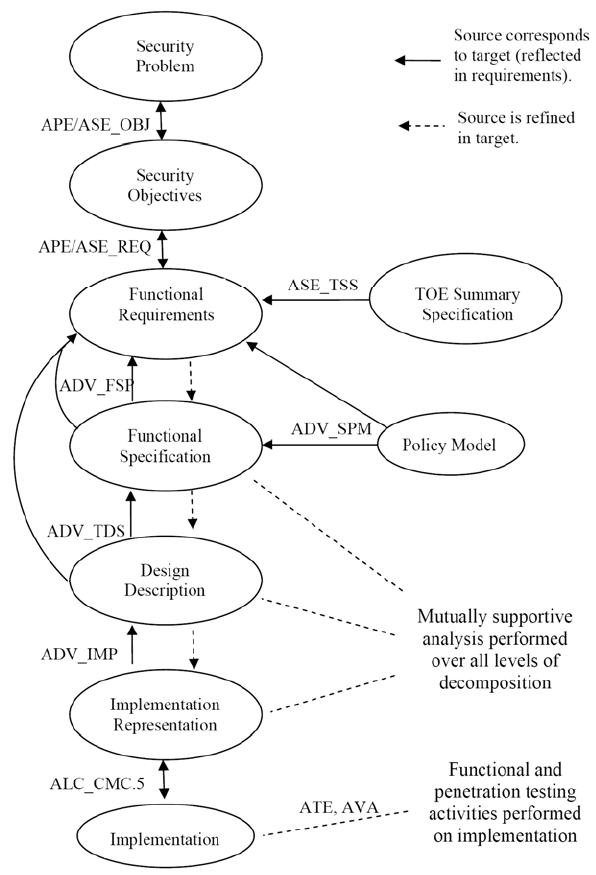
\includegraphics[keepaspectratio]{figures/layers.png}
    \caption{A TOE Security Functionality különböző absztrakciós szinteken, és a különböző rétegek
    közötti kapcsolatot biztosító követelmények.}
    \label{fig:layers}
\end{figure}
